\documentclass[twoside]{book}

% Packages required by doxygen
\usepackage{fixltx2e}
\usepackage{calc}
\usepackage{doxygen}
\usepackage[export]{adjustbox} % also loads graphicx
\usepackage{graphicx}
\usepackage[utf8]{inputenc}
\usepackage{makeidx}
\usepackage{multicol}
\usepackage{multirow}
\PassOptionsToPackage{warn}{textcomp}
\usepackage{textcomp}
\usepackage[nointegrals]{wasysym}
\usepackage[table]{xcolor}

% NLS support packages
\usepackage[spanish]{babel}
% Font selection
\usepackage[T1]{fontenc}
\usepackage[scaled=.90]{helvet}
\usepackage{courier}
\usepackage{amssymb}
\usepackage{sectsty}
\renewcommand{\familydefault}{\sfdefault}
\allsectionsfont{%
  \fontseries{bc}\selectfont%
  \color{darkgray}%
}
\renewcommand{\DoxyLabelFont}{%
  \fontseries{bc}\selectfont%
  \color{darkgray}%
}
\newcommand{\+}{\discretionary{\mbox{\scriptsize$\hookleftarrow$}}{}{}}

% Page & text layout
\usepackage{geometry}
\geometry{%
  a4paper,%
  top=2.5cm,%
  bottom=2.5cm,%
  left=2.5cm,%
  right=2.5cm%
}
\tolerance=750
\hfuzz=15pt
\hbadness=750
\setlength{\emergencystretch}{15pt}
\setlength{\parindent}{0cm}
\setlength{\parskip}{3ex plus 2ex minus 2ex}
\makeatletter
\renewcommand{\paragraph}{%
  \@startsection{paragraph}{4}{0ex}{-1.0ex}{1.0ex}{%
    \normalfont\normalsize\bfseries\SS@parafont%
  }%
}
\renewcommand{\subparagraph}{%
  \@startsection{subparagraph}{5}{0ex}{-1.0ex}{1.0ex}{%
    \normalfont\normalsize\bfseries\SS@subparafont%
  }%
}
\makeatother

% Headers & footers
\usepackage{fancyhdr}
\pagestyle{fancyplain}
\fancyhead[LE]{\fancyplain{}{\bfseries\thepage}}
\fancyhead[CE]{\fancyplain{}{}}
\fancyhead[RE]{\fancyplain{}{\bfseries\leftmark}}
\fancyhead[LO]{\fancyplain{}{\bfseries\rightmark}}
\fancyhead[CO]{\fancyplain{}{}}
\fancyhead[RO]{\fancyplain{}{\bfseries\thepage}}
\fancyfoot[LE]{\fancyplain{}{}}
\fancyfoot[CE]{\fancyplain{}{}}
\fancyfoot[RE]{\fancyplain{}{\bfseries\scriptsize Generado por Doxygen }}
\fancyfoot[LO]{\fancyplain{}{\bfseries\scriptsize Generado por Doxygen }}
\fancyfoot[CO]{\fancyplain{}{}}
\fancyfoot[RO]{\fancyplain{}{}}
\renewcommand{\footrulewidth}{0.4pt}
\renewcommand{\chaptermark}[1]{%
  \markboth{#1}{}%
}
\renewcommand{\sectionmark}[1]{%
  \markright{\thesection\ #1}%
}

% Indices & bibliography
\usepackage{natbib}
\usepackage[titles]{tocloft}
\setcounter{tocdepth}{3}
\setcounter{secnumdepth}{5}
\makeindex

% Hyperlinks (required, but should be loaded last)
\usepackage{ifpdf}
\ifpdf
  \usepackage[pdftex,pagebackref=true]{hyperref}
\else
  \usepackage[ps2pdf,pagebackref=true]{hyperref}
\fi
\hypersetup{%
  colorlinks=true,%
  linkcolor=blue,%
  citecolor=blue,%
  unicode%
}

% Custom commands
\newcommand{\clearemptydoublepage}{%
  \newpage{\pagestyle{empty}\cleardoublepage}%
}

\usepackage{caption}
\captionsetup{labelsep=space,justification=centering,font={bf},singlelinecheck=off,skip=4pt,position=top}

%===== C O N T E N T S =====

\begin{document}

% Titlepage & ToC
\hypersetup{pageanchor=false,
             bookmarksnumbered=true,
             pdfencoding=unicode
            }
\pagenumbering{roman}
\begin{titlepage}
\vspace*{7cm}
\begin{center}%
{\Large Laboratorio de P\+R\+O2. Caso de estudio\+: experimentos inmunologicos. \\[1ex]\large v7.\+0 13-\/11-\/2017 }\\
\vspace*{1cm}
{\large Generado por Doxygen 1.8.11}\\
\end{center}
\end{titlepage}
\clearemptydoublepage
\tableofcontents
\clearemptydoublepage
\pagenumbering{arabic}
\hypersetup{pageanchor=true}

%--- Begin generated contents ---
\chapter{Página principal}
\label{index}\hypertarget{index}{}El programa principal se encuentra en el módulo \hyperlink{pro2_8cc}{pro2.\+cc}.

Atendiendo a los tipos de datos sugeridos en el enunciado, necesitaremos dos módulos\+: un módulo para representar el almacén y otro para representar una sala.

La simulacion se plantea como un almacén contenedor de un conjunto de salas y un registro de productos global (incluido en el almacén). 
\chapter{Indice de archivos}
\section{Lista de archivos}
Lista de todos los archivos con descripciones breves\+:\begin{DoxyCompactList}
\item\contentsline{section}{\hyperlink{_cubeta_8hh}{Cubeta.\+hh} \\*Especificación de la clase \hyperlink{class_cubeta}{Cubeta} }{\pageref{_cubeta_8hh}}{}
\item\contentsline{section}{\hyperlink{_lavadora_8hh}{Lavadora.\+hh} \\*Especificación de la clase \hyperlink{class_lavadora}{Lavadora} }{\pageref{_lavadora_8hh}}{}
\item\contentsline{section}{\hyperlink{_prenda_8hh}{Prenda.\+hh} \\*Especificación de la clase \hyperlink{class_prenda}{Prenda} }{\pageref{_prenda_8hh}}{}
\item\contentsline{section}{\hyperlink{pro2__s8_8cc}{pro2\+\_\+s8.\+cc} \\*Programa principal para el ejercicio {\itshape Gestión de una lavadora} }{\pageref{pro2__s8_8cc}}{}
\item\contentsline{section}{\hyperlink{readbool_8hh}{readbool.\+hh} \\*Operacion para leer booleanos del canal estandar }{\pageref{readbool_8hh}}{}
\end{DoxyCompactList}

\chapter{Documentación de archivos}
\hypertarget{pro2_8cc}{}\section{Referencia del Archivo pro2.\+cc}
\label{pro2_8cc}\index{pro2.\+cc@{pro2.\+cc}}


Programa principal.  


Dependencia gráfica adjunta para pro2.\+cc\+:\nopagebreak
\begin{figure}[H]
\begin{center}
\leavevmode
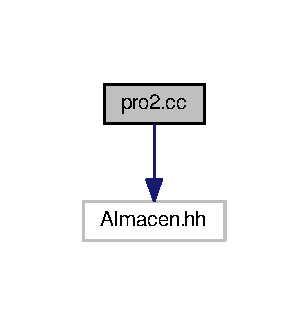
\includegraphics[width=148pt]{pro2_8cc__incl}
\end{center}
\end{figure}
\subsection*{Funciones}
\begin{DoxyCompactItemize}
\item 
int \hyperlink{pro2_8cc_ae66f6b31b5ad750f1fe042a706a4e3d4}{main} ()
\end{DoxyCompactItemize}


\subsection{Descripción detallada}
Programa principal. 

El programa incluye, para una serie de datos incorrectos específicos, un detector de error. Esto implica que si el usuario intenta realizar ciertas operaciones que no cumplan unas determinadas condiciones (como por ejemplo introducir productos no registrados) el programa informará de la existencia de un error.

Pese a lo previamente citado, suponemos que el usuario introduce datos correctos relativos al acceso a salas ya que no hay control respecto a si accedemos a salas inexistentes o se introducen cantidades negativas. 

\subsection{Documentación de las funciones}
\index{pro2.\+cc@{pro2.\+cc}!main@{main}}
\index{main@{main}!pro2.\+cc@{pro2.\+cc}}
\subsubsection[{\texorpdfstring{main()}{main()}}]{\setlength{\rightskip}{0pt plus 5cm}int main (
\begin{DoxyParamCaption}
{}
\end{DoxyParamCaption}
)}\hypertarget{pro2_8cc_ae66f6b31b5ad750f1fe042a706a4e3d4}{}\label{pro2_8cc_ae66f6b31b5ad750f1fe042a706a4e3d4}


Definición en la línea 31 del archivo pro2.\+cc.


\begin{DoxyCode}
31            \{
32 
33   \textcolor{keywordtype}{int} N;                \textcolor{comment}{// Cantidad de salas.}
34   cin >> N;
35   
36   \hyperlink{class_almacen}{Almacen} A(N);            \textcolor{comment}{// Creación y lectura en preorden de la estructura del almacén (con
       identificadores de sala).}
37   
38   A.lectura\_dimensiones\_salas();    \textcolor{comment}{// Lectura de las dimensiones de cada una de las salas.}
39   
40   \textcolor{keywordtype}{string} op;              \textcolor{comment}{// Código de operación.}
41   
42   \textcolor{keywordflow}{while} (cin >> op and op != \textcolor{stringliteral}{"fin"}) \{
43     
44     cout << op;
45     
46     \textcolor{keywordflow}{if} (op == \textcolor{stringliteral}{"poner\_prod"}) \{
47       \textcolor{keywordtype}{string} prod;
48       cin >> prod;
49       
50       cout <<\textcolor{charliteral}{' '} << prod << endl;
51       A.poner\_prod(prod);
52     \}
53     \textcolor{keywordflow}{else} \textcolor{keywordflow}{if} (op == \textcolor{stringliteral}{"quitar\_prod"}) \{
54       \textcolor{keywordtype}{string} prod;
55       cin >> prod;
56       
57       cout <<\textcolor{charliteral}{' '} << prod << endl;
58       A.quitar\_prod(prod);
59     \}
60     \textcolor{keywordflow}{else} \textcolor{keywordflow}{if} (op == \textcolor{stringliteral}{"poner\_items"}) \{
61       \textcolor{keywordtype}{int} sala, cant;
62       \textcolor{keywordtype}{string} prod;
63       cin >> sala >> prod >> cant;
64       
65       cout <<\textcolor{charliteral}{' '} << sala << prod << cant << endl;
66       
67       \textcolor{keywordtype}{int} result = A.poner\_items(sala, prod, cant);
68       \textcolor{keywordflow}{if} (result == -1) cout << \textcolor{stringliteral}{"  error"} << endl;
69       \textcolor{keywordflow}{else} cout <<\textcolor{stringliteral}{"  "} << result << endl;
70     \}
71     \textcolor{keywordflow}{else} \textcolor{keywordflow}{if} (op == \textcolor{stringliteral}{"quitar\_items"}) \{
72       \textcolor{keywordtype}{int} sala, cant;
73       \textcolor{keywordtype}{string} prod;
74       cin >> sala >> prod >> cant;
75       
76       cout <<\textcolor{charliteral}{' '} << sala << prod << cant << endl;
77       
78       \textcolor{keywordtype}{int} result = A.quitar\_items(sala, prod, cant);
79       \textcolor{keywordflow}{if} (result == -1) cout << \textcolor{stringliteral}{"  error"} << endl;
80       \textcolor{keywordflow}{else} cout <<\textcolor{stringliteral}{"  "} << result << endl;
81       
82     \}
83     \textcolor{keywordflow}{else} \textcolor{keywordflow}{if} (op == \textcolor{stringliteral}{"distribuir"}) \{
84       \textcolor{keywordtype}{int} cant;
85       \textcolor{keywordtype}{string} prod;
86       cin >> prod >> cant;
87       
88       cout <<\textcolor{charliteral}{' '} << prod << cant << endl;
89       
90       \textcolor{keywordtype}{int} result = A.distribuir(prod, cant);
91       \textcolor{keywordflow}{if} (result == -1) cout << \textcolor{stringliteral}{"  error"} << endl;
92       \textcolor{keywordflow}{else} cout <<\textcolor{stringliteral}{"  "} << result << endl;
93       
94     \}
95     \textcolor{keywordflow}{else} \textcolor{keywordflow}{if} (op == \textcolor{stringliteral}{"compactar"}) \{
96       \textcolor{keywordtype}{int} sala;
97       cin >> sala;
98       
99       cout <<\textcolor{charliteral}{' '} << sala << endl;
100       A.compactar(sala);
101     \}
102     \textcolor{keywordflow}{else} \textcolor{keywordflow}{if} (op == \textcolor{stringliteral}{"reorganizar"}) \{
103       \textcolor{keywordtype}{int} sala;
104       cin >> sala;
105       
106       cout <<\textcolor{charliteral}{' '} << sala << endl;
107       A.reorganizar(sala);
108     \}
109     \textcolor{keywordflow}{else} \textcolor{keywordflow}{if} (op == \textcolor{stringliteral}{"redimensionar"}) \{
110       \textcolor{keywordtype}{int} sala, fil, col;
111       cin >> sala >> fil >>col;
112       
113       cout <<\textcolor{charliteral}{' '} << sala << fil << col << endl;
114       \textcolor{keywordflow}{if} (not A.redimensionar(sala, fil, col)) cout << \textcolor{stringliteral}{"  error"} << endl;
115     \}
116     \textcolor{keywordflow}{else} \textcolor{keywordflow}{if} (op == \textcolor{stringliteral}{"inventario"}) \{
117       
118       A.inventario();
119     \}
120     \textcolor{keywordflow}{else} \textcolor{keywordflow}{if} (op == \textcolor{stringliteral}{"escribir"}) \{
121       \textcolor{keywordtype}{int} sala;
122       cin >> sala;
123       
124       cout <<\textcolor{charliteral}{' '} << sala << endl;
125       A.escribir(sala);
126     \}
127     \textcolor{keywordflow}{else} \textcolor{keywordflow}{if} (op == \textcolor{stringliteral}{"consultar\_pos"}) \{
128       \textcolor{keywordtype}{int} sala, fil, col;
129       cin >> sala >> fil >>col;
130       
131       cout <<\textcolor{charliteral}{' '} << sala << fil << col << endl;
132       cout <<\textcolor{stringliteral}{"  "} << A.consultar\_pos(sala, fil, col) << endl;
133     \}
134     \textcolor{keywordflow}{else} \textcolor{keywordflow}{if} (op == \textcolor{stringliteral}{"consultar\_prod"}) \{
135       \textcolor{keywordtype}{string} prod;
136       cin >> prod;
137       
138       cout <<\textcolor{charliteral}{' '} << prod << endl;
139       \textcolor{keywordtype}{int} result = A.consultar\_prod(prod);
140       
141       \textcolor{keywordflow}{if} (result == -1) cout << \textcolor{stringliteral}{"  error"} << endl;
142       \textcolor{keywordflow}{else} cout <<\textcolor{stringliteral}{"  "} << result << endl;
143     \}
144   \}
145   
146   cout << op << endl;
147 \}
\end{DoxyCode}

%--- End generated contents ---

% Index
\backmatter
\newpage
\phantomsection
\clearemptydoublepage
\addcontentsline{toc}{chapter}{Índice}
\printindex

\end{document}
